% !TEX root = extra-answers.tex
\chead{\textbf{Unused exercises}}

\begin{document}

\begin{enumerate}
	\item
	It is known that men that are overweight are at high risk of contracting COVID19 and then needing intensive care. We assume that the population consists of 50\% men and 50\% woman and that half of each group is overweight. Clearly, gender is independent from being overweight. Still, when visiting an intensive care unit, one may find a higher proportion of men among the patients with a healthy weight than among the overweight patients. This is an example of the ``explain away'' effect, which occurs when the graphical model is a collider.

	We have three Boolean variables: whether the patient is male ($M$), overweight ($O$) and in need of intensive care ($C$). Given the assumption that $M$ and $O$ are independent, we can system with following graphical model:
	\begin{equation*}
		\begin{tikzpicture}[scale=1, transform shape]
			\tikzstyle{every node} = [draw,shape=circle]
			\node (M) at (0,0) {$M$};
			\node (O) at (3,0) {$O$};
			\node (C) at (1.5,-1) {$C$};
			\draw[-{Latex[length=3mm, width=2mm]}] (M) to (C);
			\draw[-{Latex[length=3mm, width=2mm]}] (O) to (C);
		\end{tikzpicture}
	\end{equation*}
	This model simply represents the fact that the joint probability $P(M, O, C)$ distribution can be factorised as:
	\[
		P(M, O, C) = P(M)P(O)P(C|M, O)
	\]
	Because this is a collider, we have that while $M$ and $O$ are independent, $M$ and $O$ become dependent when conditioning on $C$. We study this in the particular case with conditional probability distributions:
	\begin{align*}
		P(M=1)=P(O=1)                 & =1/2  \\
		P(C=1|M=0, O=0)               & = 1/4 \\
		P(C=1|M=1, O=0)=P(C|M=0, O=1) & = 1/2 \\
		P(C=1|M=1, O=1)               & =3/4
	\end{align*}

	Use basic probability rules to give the probability $P(M=1 | O=1, C=1)$ that an overweight patient in need of intensive care is male and the probability $P(M=1 | O=0, C=1)$ that a not-overweight patient in need of intensive care is male. (4pts)

	\begin{gradedsolution}
		\begin{align*}
			P(M=1, O=1, C=1)=3/4 \times 1/4 & =3/16 \\
			P(M=0, O=1, C=1)=1/2 \times 1/4 & =2/16 \\
			P(M=1|O=1,C=1)                  & =3/5  \\
			P(M=1, O=0, C=1)=2/4 \times 1/4 & =2/16 \\
			P(M=0, O=0, C=1)=1/4 \times 1/4 & =1/16 \\
			P(M=1|O=0,C=1)                  & =2/3  \\
		\end{align*}
	\end{gradedsolution}

	\item (1 point) $\Zcal, \Tcal, \Wcal$ are assumed to be finite discrete spaces with Markov kernels:\\

	\[Q(Z|W):\, \Wcal \dshto \Zcal,\quad (C,w) \mapsto Q(Z \in C|W=w),  \]
	\[K(W|T):\, \Tcal \dshto \Wcal,\quad (D,t) \mapsto K(W \in D|T=t),  \]

	and corresponding stochastic matrices:

	\[\tilde Q =
		\begin{bmatrix}
			0.1 & 0.7 & 0.2 \\
			0.3 & 0   & 0.4 \\
			0.6 & 0.3 & 0.4 \\
		\end{bmatrix}
		\qquad
		\tilde K =
		\begin{bmatrix}
			0.2 & 0.1 & 0.6 \\
			0.3 & 0.1 & 0   \\
			0.5 & 0.8 & 0.4 \\
		\end{bmatrix}\]


	Compute the stochastic matrix $\tilde P$ for the composed  Markov kernel: $P(Z|T):=Q(Z|W) \circ K(W|T)$.

	\begin{gradedsolution}
		$\tilde P = \begin{bmatrix}
				0.33 & 0.24 & 0.14 \\
				0.26 & 0.35 & 0.34 \\
				0.41 & 0.41 & 0.52 \\
			\end{bmatrix}$.
	\end{gradedsolution}

	\item %\textbf{BONUS} 
	Provide an example of Markov kernels
	\begin{align*}
		X : \Wcal \times \Tcal \rightarrow \Xcal, \quad Y : \Wcal \times \Tcal \rightarrow \Ycal, \quad Z : \Wcal \times \Tcal \rightarrow \Zcal
	\end{align*}
	such that $$X \Indep_{K(W|T)} Y \given Z \quad \text{but} \quad Y \nIndep_{K(W|T)} X \given Z.$$
	\begin{ungradedsolution}
		Given $\Tcal := \{0,1\}$, standard measurable space $\Xcal$ and distribution $\mathbb{P}(X)$, define Markov kernel $K(X|T):=\mathbb{P}(X)$. Consider
		\begin{align*}
			X & : \Wcal \times \Tcal \rightarrow \Xcal \quad \text{constant in $\Tcal$} \\
			T & :\Wcal\times \Tcal \rightarrow \Tcal, \quad (w, t) \mapsto t            \\
			* & : \Wcal \times \Tcal \rightarrow \{*\}, \quad (w, t) \mapsto *,
		\end{align*}
		then we have $X\Indep T|*$ since
		\begin{align*}
			K(X, T, *|T) = Q(X|*) \otimes K(T, *|T)
		\end{align*}
		for $Q(X|*) := \mathbb{P}(X)$.  However, $T\nIndep X|*$ since there can be no $Q(*|X)$ (which is equal to 1 for all $x\in\Xcal$) such that $K(T, X, *|T) = Q(*|X)\otimes K(X, *|T)$, as
		$$K(T, X, *|T) = \delta(T|T)\otimes K(X|T) = \delta(T|T)\otimes \mathbb{P}(X)$$
		and
		$$Q(*|X)\otimes K(X, *|T) = 1\otimes K(X|T) = \mathbb{P}(X).$$
	\end{ungradedsolution}

	\item
	$d$-separation is defined for walks as follows: ... Show that this is an equivalent definition to the definition of $d$-separation for walks.
	\item
	Prove Reichenbach's principle using the Global Markov Property: $X\nIndep Y\implies X\to Y, X\leftarrow Y$ or $X\leftrightarrow Y$.
	\item %(\textbf{BONUS})
	Prove Lemma \ref*{lem:stability_separation_marginalization} for $d$-separation: show that $d$-separation holds in the marginalised graph if and only if it holds in the full graph.
	\item %($3 \times 1$ points)
	Provide an example of a real-world system, give an example of:
	\begin{enumerate}
		\item a soft intervention
		\item a hard intervention
		% \item a node-splitting intervention
	\end{enumerate}
	on this system and draw the CDMGs related to these interventions.
	\emph{Hint: When drawing the CDMG related to a (intervened) system, give appropriate names to the variables involved, and provide explicit descriptions of these variables. Also, make sure that all the variables and causal mechanisms that occur in the description of the system are represented in the graph.}
	\item
	Write a program in R or Python\footnote{We recommend using R, since this is likely the more suitable programming language for the project later in the course. As an introduction, you could take a look at https://cran.r-project.org/doc/manuals/r-release/R-intro.pdf or any of the many tutorials in the internet.} for the structural causal model which is described by the equation
	\begin{equation*}
		N \leftarrow \gamma + \delta C,
		\label{eq:chocolate_causes_nobel}
	\end{equation*}
	(treating $C$ as an exogenous input, and $N$ as endogenous)
	analogous to the program in Figure 4 of the lecture notes.
	In your program, simulate from the model in the observational setting, after the hard intervention
	do$(C = c)$, and after the hard intervention do$(N = n)$.
	As your answer, copy-paste your code and the output of the program.
	\begin{gradedsolution}
		This is our code:
		\begin{figure}[H]
			\centering
			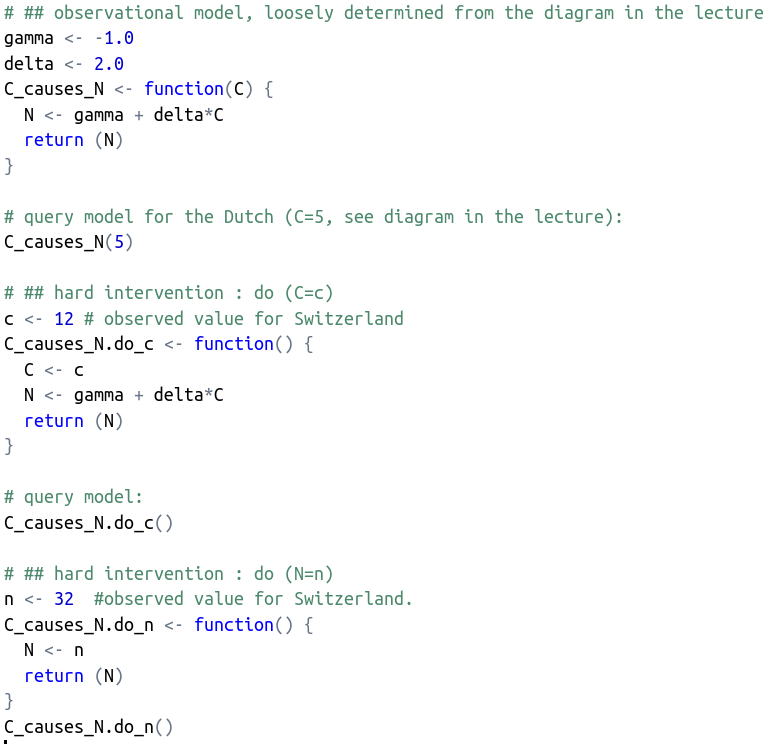
\includegraphics[width=0.8\textwidth]{r_code}
		\end{figure}
		This is the output of the code:
		\begin{figure}[H]
			\centering
			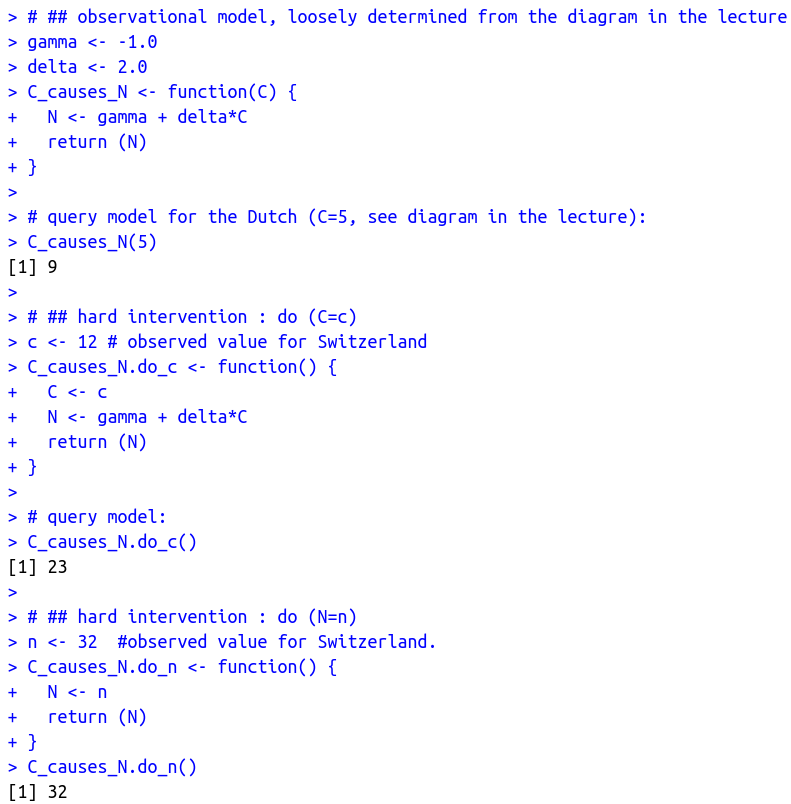
\includegraphics[width=0.8\textwidth]{r_output}
		\end{figure}
	\end{gradedsolution}

	\item Consider the following set of structural equations:
	\begin{align}
		Z & = U + V \cdot X \\
		V & = 2 X           \\
		U & = Y - X         \\
		X & = 3 Y - 4
		\label{eq:acyclic_structural_equations}
	\end{align}
	where all the variables $X, Z, U, V, Y$ take values in $\mathbb{R}$.
	We assume that $U,V,X,Z$ are endogenous and $Y$ is an exogenous input variable in this model.\\
	\textcolor{red}{Feedback: I forgot to specify that the solution function should be "completely computed", i.e. there should not be non-evaluated functions anymore in the solution function.}\\
	\textcolor{red}{Feedback: The notation is bad, since the Y variable is part of curly X, and the X and Z variables are part of curly Y. Definitely needs to be changed, since students were somewhat confused.}\\
	\textcolor{red}{Feedback: The definition / notation etc. of SCMs changed throughout the lecture, and so the notations / definitions in this third exercise sheet are no longer valid.}\\
	Do the following exercises:
	\begin{enumerate}
		\item Find a formal structural causal model $\mathcal{M} = \left\langle \boldsymbol{\mathcal{X}}, \boldsymbol{\mathcal{Y}}, \boldsymbol{\mathcal{Z}}, P, \boldsymbol{f}\right\rangle$ that represents the structural equations above.
		\item Let $(f_W)_{W \in \{X,Z,U,V\}}$ be the components of the causal mechanism function $\boldsymbol{f}$ you found in the exercise above.
		Show that there is a \emph{topological ordering} of the variables $\{Z,X,U,V\}$, meaning that it is possible to order them in such a way that each component $f_W$ depends only on variables that appear before $W$ in the ordering.
		Formally, this means finding a bijection $\sigma: \{X, Z, U, V\} \to \{1, 2, 3, 4\}$ such that $f_{W}$ does not depend on $W'$ if $\sigma(W) \leq \sigma(W')$.
		\item With the help of your topological ordering, find a solution function $\boldsymbol{g}: \boldsymbol{\mathcal{X}} \times \boldsymbol{\mathcal{Z}} \to \boldsymbol{\mathcal{Y}}$ for $\mathcal{M}$:
		First, explain intuitively how one can find a solution. Then, write it down formally in the form of a function $\boldsymbol{g}$.
		Finally, formally verify that it is a solution function by showing that the structural equation $\boldsymbol{g}(\boldsymbol{x}, \boldsymbol{z}) = \boldsymbol{f}(\boldsymbol{x}, \boldsymbol{g}(\boldsymbol{x}, \boldsymbol{z}), \boldsymbol{z})$ is satisfied for all $\boldsymbol{x} \in \boldsymbol{\mathcal{X}}$ and almost all $\boldsymbol{z} \in \boldsymbol{\mathcal{Z}}$.
		\item Explain intuitively why $\boldsymbol{g}$ found above is the \emph{unique} solution function, see Definition 5.7.1. This does not need to be a formal proof.
		If you are comfortable with giving proofs, however, you can also give a proof instead of an intuitive explanation.
		\item Give an example of a structural causal model $\mathcal{M}'$ which can not be topologically ordered in this sense.
		%    In order to complicate this task, we ask you that if $f'_{j_1}$ depends on $Y'_{j_2}$ in your model, that then $f'_{j_2}$ does not depend on $Y'_{j_1}$.
		\item Does your new model have a solution function? If so, is it unique? Explain.
	\end{enumerate}
	\begin{gradedsolution}
		\begin{enumerate}
			\item $\boldsymbol{\mathcal{X}} = \mathbb{R}$, $\boldsymbol{\mathcal{Y}} = \mathbb{R}^{4}$\footnote{Sorry for the notation: this is consistent with the lecture, but of course, $\mathbf{\mathcal{X}}$ contains elements $y$ corresponding to the variable $Y$, etc.}, $\boldsymbol{\mathcal{Z}} = \{*\}$, the one-point-set, $P: \{\emptyset, \boldsymbol{\mathcal{Z}}\} \to [0,1]$ is given by $P = \delta_{*}$, the Dirac measure of the only point, and, finally, $\boldsymbol{f}: \boldsymbol{\mathcal{X}} \times \boldsymbol{\mathcal{Y}} \times \boldsymbol{\mathcal{Z}} = \mathbb{R}^{5} \to \mathbb{R}^{4} = \boldsymbol{\mathcal{Y}}$\footnote{In the identification $\boldsymbol{\mathcal{X}} \times \boldsymbol{\mathcal{Y}} \times \boldsymbol{\mathcal{Z}} = \mathbb{R}^{5}$ we use the typical convention that $U \times \{*\} = U$, even though, technically, this is only an isomorphism and not an equality} is given by:
			\begin{equation}
				f \begin{pmatrix} y \\ x \\ u \\ v \\ z\end{pmatrix}
				= \begin{pmatrix} 3y - 4 \\ y - x \\ 2x \\ u + v \cdot x\end{pmatrix}
				\label{eq:functional_equation}
			\end{equation}
			which we have already conveniently ordered.
			\item They already are topologically ordered. Formally, we have $\sigma(X) = 1$, $\sigma(U) = 2$, $\sigma(V) = 3$, and $\sigma(Z) = 4$.
			\item Intuition: We need to find a solution function $g: \boldsymbol{\mathcal{X}} \times \boldsymbol{\mathcal{Z}} = \mathbb{R} \to \boldsymbol{\mathcal{Y}} = \mathbb{R}^{4}$ such that the equation
			\begin{align}
				\begin{split}
					\begin{pmatrix} g_X(y) \\ g_U(y) \\ g_V(y) \\ g_Z(y)\end{pmatrix} & = \boldsymbol{g}(y)  = \boldsymbol{g}(\boldsymbol{x}, \boldsymbol{z}) = \boldsymbol{f}(\boldsymbol{x}, \boldsymbol{g}(\boldsymbol{x}, \boldsymbol{z}), \boldsymbol{z})
					\\ &	  = \boldsymbol{f}(y, \boldsymbol{g}(y))  =
					f \begin{pmatrix} y \\ g_X(y) \\ g_U(y) \\ g_V(y) \\ g_Z(y)\end{pmatrix} = \begin{pmatrix} 3y - 4 \\ y - g_X(y) \\ 2g_X(y) \\ g_U(y) + g_V(y) \cdot g_X(y)\end{pmatrix}
				\end{split}
				\label{eq:eq_constraint}
			\end{align}
			holds.
			Comparing the left and the right side, we get the four equations $g_X(y) = 3y - 4$, $g_U(y) = y - g_X(y)$, $g_V(y) = 2g_X(y)$, $g_Z(y) = g_U(y) + g_V(y) \cdot g_X(y)$.
			Now, we see what the topological ordering is there for: We can solve these equations one-by-one from left to right, since the ordering then ensures that all the parts which we need for computing the next component-function of $\boldsymbol{g}$ has already been computed.
			We can also imagine the variables $Y, X, U, V, Z$ to be arranged in a graph with an arrow $W \to W'$ whenever one needs $W$ in order to determine $W'$. Then, with these equations we can ``propagate forward'' the solution along the graph.
			If we do this, we end up with the following solution function:
			\begin{equation}
				\boldsymbol{g}(y) = \begin{pmatrix} 3y - 4 \\ -2y + 4 \\ 6y - 8 \\ 18y^{2} - 50y + 36\end{pmatrix}.
				\label{eq:the_solution_function}
			\end{equation}
			Finally, we need to show that this satisfies the structural equation.
			This holds of course by construction, but here is the formal proof:
			\begin{align*}
				\boldsymbol{f}(y, \boldsymbol{g}(y)) & = f
				\begin{pmatrix} y \\ 3y - 4 \\ -2y + 4 \\ 6y - 8 \\ 18y^{2} - 50y + 36\end{pmatrix}
				= \begin{pmatrix} 3y - 4 \\ y - (3y - 4) \\ 2(3y - 4) \\ -2y + 4 + (6y - 8) \cdot (3y - 4)\end{pmatrix}                  \\
				                                     & = \begin{pmatrix} 3y - 4 \\ -2y + 4 \\ 6y - 8 \\ 18y^{2} - 50y + 36 \end{pmatrix}
				= \boldsymbol{g}(y),
				\label{eq:verify_solution}
			\end{align*}
			which verifies the solution.
			\item In Equation \eqref{eq:eq_constraint}, we assumed that $\boldsymbol{g}$ satisfies the constraint and then ended up with four equations that forced us, one by one, to write down the solution function that we found.
			This already proves uniqueness.
			\item We set $\boldsymbol{\mathcal{X}}' = \{*\}$, $\boldsymbol{\mathcal{Y}}' = \mathbb{R}$, $\boldsymbol{\mathcal{Z}}' = \{*\}$, $P' = \delta_{*}$, and $\boldsymbol{f}': \boldsymbol{\mathcal{Y}}' \to \boldsymbol{\mathcal{Y}}'$, $\boldsymbol{f}'(y) = y$.
			\item For any $y_* \in \mathbb{R}$, the function $\boldsymbol{g}_{y_*}: \boldsymbol{\mathcal{X}} \times \boldsymbol{\mathcal{Z}} = \{*\} \to \boldsymbol{\mathcal{Y}} = \mathbb{R}$ given by $\boldsymbol{g}_{y_*}(*) = y_*$ is a solution, since $\boldsymbol{f}(\boldsymbol{g}_{y_*}(*)) = \boldsymbol{g}_{y_*}(*)$ by definition of $\boldsymbol{f}$.
			Thus, there are infinitely many solutions.
			Intuitively, this is due to a ``cycle'' (to be defined in the lecture) in the corresponding causal graph.
		\end{enumerate}
	\end{gradedsolution}

	\item We call an SCM $\C{M}=\langle \Sin, \Send, \Srnd, \CX, P, f \rangle$
	\emph{linear} if all variables are real-valued and
	each component of the causal mechanism is a linear combination of variables, that is
	$$
		f_v(x) = \sum_{w\in V \cup J \cup W} B_{vw} x_w,
	$$
	where $B\in\RN^{V \times (V \cup J \cup W)}$ is a matrix of coefficients.

	\begin{enumerate}
		\item Show that for any set $L \subseteq V$, $(\C{M})_{\doit(V\setminus L)}$ is uniquely solvable if and only if the matrix $I_{L}-B_{LL}$ is invertible. Give the unique solutions function. (1pt)
		\item Bonus: generalize and prove this statement for non-linear SCMs and invertible non-linear functions. (1pt)
	\end{enumerate}

	\item For a simple SCM $\C M$ and a subset $L \subset V$ of endogenous variables, we have $G(\C M_{\setminus L}) \subseteq G(\C M)^{\setminus L}$. Construct a simple SCM and a subset $L$ for which $G(\C M_{\setminus L}) \neq G(\C M)^{\setminus L}$ and explain why. (1pt)

	\item Equivalence of SCMs is preserved by twinning. \textbf{(1pt)}
	\begin{gradedsolution}
		Let $\mathcal{M} \equiv \widetilde{\mathcal{M}}$. Let the twinned SCMs be given by
		\begin{align*}
			\mathcal{M}^{\text{twin}}             & = \left\langle J \cup J', V \cup V', W, \mathcal{X}^{\text{twin}}, P, f \times f' \right\rangle                          \\
			\widetilde{\mathcal{M}}^{\text{twin}} & = \left\langle J \cup J', V \cup V', W, \mathcal{X}^{\text{twin}}, P, \widetilde{f} \times \widetilde{f}' \right\rangle,
		\end{align*}
		where we set $\mathcal{X}^{\text{twin}} = \mathcal{X}_J \times \mathcal{X}_{J} \times \mathcal{X}_{V} \times \mathcal{X}_V \times \mathcal{X}_W$, and where $f \times f'$ is given by
		\begin{equation*}
			(f \times f')(x_J, x_{J'}, x_V, x_{V'}, x_W) = (f(x_J, x_V, x_W), f(x_{J'}, x_{V'}, x_W)) \in \mathcal{X}_V \times \mathcal{X}_{V}.
		\end{equation*}
		$\widetilde{f} \times \widetilde{f}'$ is constructed in the same way.

		Then, for arbitrary $v \in V$ and $x \in \mathcal{X}^{\text{twin}}$ we obtain:
		\begin{align*}
			x_v = (f \times f')_v(x_J, x_{J'}, x_V, x_{V'}, x_W) & \Longleftrightarrow x_v = f_v(x_J, x_V, x_W)                                                    \\
			                                                     & \Longleftrightarrow x_v = \widetilde{f}_v(x_J, x_V, x_W)                                        \\
			                                                     & \Longleftrightarrow x_v = (\widetilde{f} \times \widetilde{f}')(x_J, x_{J'}, x_V, x_{V'}, x_W).
		\end{align*}
		The same arguments work if $v \in V'$, and thus we are done and have shown that the twinned SCMs are still equivalent.
	\end{gradedsolution}

	\item %(3 points)
	      (\textbf{Note that this is proven in Propositions \ref*{prp:pearls_ladder_levels_1_and_2} and \ref*{prp:pearls_ladder_levels_2_and_3}})
	In this exercise, we prove parts of the ``Ladder of Causation'', which, roughly speaking, comes down to the insight that modeling interventions is more expressive than just modeling observations, and that modeling counterfactuals is more expressive than just modeling interventions.
	Part of this is displayed in Proposition \ref*{prp:pearls_ladder_levels_2_and_3} in the lecture notes.

	Let $M$ and $\tilde{M}$ be two simple SCMs and $O \subseteq (V \cap \tilde{V}) \cup (W \cap \tilde{W})$.
	Prove the following:
	\begin{enumerate}
		\item If $M \equiv \tilde{M}$ then $M$ and $\tilde{M}$ are counterfactually equivalent with respect to $O$.
		\item If $M$ and $\tilde{M}$ are counterfactually equivalent with respect to $O$, then $M$ and $\tilde{M}$ are interventionally equivalent with respect to $O$.
		\item If $M$ and $\tilde{M}$ are interventionally equivalent with respect to $O$, then $M$ and $\tilde{M}$ are observationally equivalent with respect to $O$.
	\end{enumerate}

	\begin{ungradedsolution}
		\begin{enumerate}
			\item Assume $M \equiv \tilde{M}$.
			By Proposition \ref*{prp:twinning_preserves_scm_equivalence} this implies that $M^{\text{twin}} \equiv \tilde{M}^{\text{twin}}$.
			From Exercise 1.b of week 10, we obtain $\left( M^{\text{twin}}\right)_{\doit(T)} \equiv \left( \tilde{M}^{\text{twin}}\right)_{\doit(T)} $ for all $T \subseteq J \cup J' \cup V \cup V' \cup W$.
			This then also holds for all $T \subseteq O \cup O'$.
			From Exercise 1.d of week 10, we then obtain that for all these $T$, $\left( M^{\text{twin}}\right)_{\doit(T)} $ and $\left( \tilde{M}^{\text{twin}}\right)_{\doit(T)} $ have the same Markov kernels.
			Marginalizing these Markov kernels, and only keeping the variables $X_{O \cup O' \setminus T}$ in them, this implies observational equivalence of $\left( M^{\text{twin}}\right)_{\doit(T)} $ $\left( \tilde{M}^{\text{twin}}\right)_{\doit(T)} $ with respect to $O \cup O' \setminus T$.
			Since this holds for all $T \subseteq O \cup O'$, this implies interventional equivalence of $M^{\text{twin}}$ and $\tilde{M}^{\text{twin}}$ with respect to $O \cup O'$.
			This, in turn, is counterfactual equivalence of $M$ and $\tilde{M}$ with respect to $O$.
			Thus, we are done.
			\item First we note that for $M^\twin = \lt \Sin \dot\cup \Sin', \Send \dot\cup \Send', \Srnd, \tilde{\CX}, P, \tilde{f} \rt$, we have the marginalised SCM $M^\twin_{\setminus \Send'} = \lt \Sin \dot\cup \Sin', \Send, \Srnd, \CX_{\Sin'}\times \CX, P, f \rt$. As there are no edges pointing towards $J'$ and $W$ and there are no directed paths from $V'$ to $J\cup V\cup W$ in $G(M^\twin)$, the nodes $J'$ are disconnected from all other nodes ($J\cup V\cup W$) in $G(M^\twin_{\setminus \Send'})$. Therefore, for all $A\subseteq V\cup W$ and $D\subseteq V\cup W$ we have $A\perp^\sigma J' | D\cup J$ in $G((M^\twin_{\setminus \Send'})_{\doit(D)})$, so by the first rule of do calculus we have
			$$P(X_A | \doit(X_{D\cup J \cup J'})) = P(X_A | \doit(X_{D\cup J})).$$
			Hence, the SCMs $M^\twin_{\setminus \Send'}$ and $M := \lt \Sin, \Send, \Srnd, \CX, P, f \rt$ are interventionally equivalent with respect to $V\cup W$.


			Now, let $M$ and $\tilde{M}$ be counterfactually equivalent with respect to $O$. Then, by definition, the SCMs $M^\twin$ and $\tilde{M}^\twin$ are interventionally equivalent with respect to $O\cup O'$. By Corollary \ref*{Cor:various_equiv_marginalization}, the SCMs $M^\twin_{\setminus V'}$ and $\tilde{M}^\twin_{\setminus \tilde{V}'}$ are interventionally equivalent with respect to $O$. By the above argument, the former and the latter are respectively interventionally equivalent to $M$ and $\tilde{M}$ with respect to $O$. By transitivity of interventional equivalence, we conclude that $M$ and $\tilde{M}$ are interventionally equivalent with respect to $O$.


			\item That $M$ and $\tilde{M}$ are interventionally equivalent with respect to $O$ means that, for all $T \subseteq O$, $M_{\text{do}(T)}$ is observationally equivalent to $\tilde{M}_{\text{do}(T)}$ with respect to $O \setminus T$.
			Setting $T = \emptyset$ implies that $M$ and $\tilde{M}$ are observationally equivalent with respect to $O$.
		\end{enumerate}
	\end{ungradedsolution}

	\item (2 points) By marginalizing out all variables in $V \cup W$ except $a$ and $b$, give short proofs of:
	\begin{enumerate}
		\item Proposition \ref*{prp:scm_causes_separation}: Let $M = \langle \Sin, \Send, \Srnd, \CX, P, f \rangle$ be a simple SCM with graph $G = G(M)$.
		Let $a \in V \cup W \cup J$ and $b \in V$.
		If $a \notin \Anc^G(b)$, then:
		$$P_{M}(X_b \given \doit(X_{J\cup \{a\}})) = P_{M}(X_b \given \doit(X_{J\setminus \{a\}})).$$
		\item Proposition \ref*{prp:scm_confounded_separation}:  Let $M = \lt \Sin, \Send, \Srnd, \CX, P, f \rt$ be a simple SCM with graph $G = G(M)$.
		Let $a \ne b \in V$.
		If $b \notin \Anc^G(a)$ and $a$ and $b$ do not have a common cause according to $M$, then
		$a$ and $b$ do not have confounding bias:
		$$P_{M}(X_b \given \doit(X_a), \doit(X_J)) = P_{M}(X_b \given X_a, \doit(X_J)).$$
	\end{enumerate}

	\begin{gradedsolution}
		\begin{enumerate}
			\item After marginalization we only retain variables $a$ and $b$ and all variables in $J$. Let us first consider the case $a \in V \cup W$. We will show that
			$$b \Perp^\sigma_{G_{\doit(I_a)}} I_a \mid J \setminus \{a\}.$$
			Since $a$ is not an ancestor of $b$ and all edges from $J$ are outgoing, $a$ can only have incoming edges. Consider a walk from $b$ to $I_a \cup J$. Any walk from $b$ to $J$ is $\sigma$-blocked since we condition on the end points. Any walk from $b$ to $I_a$ must go through $a$, which is a collider since it only has incoming edges and is not conditioned on. Therefore the separation holds.
			Now consider the case $a \in J$. We will show that
			$$b \Perp^\sigma_{G} a \mid J \setminus \{a\}.$$
			Since $a \in J$, the only possible edge from $a$ is an edge to the only non-input variable $b$. But since $a \notin \Anc^G(b)$, $a$ has no edges. Consider a walk from $b$ to $J$. The node $a$ can not be an endpoint since it has no edges. On the other hand if the end point is in $J \setminus \{a\}$ it is $\sigma-$blocked by our conditioning. Thus the $\sigma$-separation holds.\\
			In both cases, rule 3 of do-calculus yields the result.
			\item After marginalization we only retain variables $a$ and $b$ and all variables in $J$. We will show that the assumptions imply $b \Perp^\sigma_{G_{\doit(I_a)}} I_a \given \{a\} \cup J$.

			Since $b \notin \Anc^G(a)$ and $a$ and $b$ are not confounded, the we have either $a \to b$ or no edge between $a$ and $b$. Consider a walk in $G_{\doit(I_a)}$ between $b$ and $I_a \cup J$. It cannot contain nodes from $J$ as such a node would either be an end node of the walk ($\sigma$-blocking it) or a non-collider node pointing only to nodes in another strongly connected component of $G_{\doit(I_a)}$
			($\sigma$-blocking the walk). Thus the only possible walk is $I_a \to a \to b$, which is $\sigma$-blocked by conditioning on $a$. Hence the $\sigma$-separation holds.

			Invoking rule 2 of the do-calculus then yields the result.
		\end{enumerate}
	\end{gradedsolution}

\end{enumerate}
\end{document}
